\section{Bargaining about another player's opportunities}
\label{sec:bargaining}

\subsection{Responses and the composition of offers}
Across 526 negotiation threads, players accept 113 offers, counter 394 and reject 413. Acceptance is legal in 918 of the 920 response opportunities. Sol and Opus counter most frequently, whereas Gemini and Grok reject most frequently. Each nevertheless accepts between 26 and 30 offers. Those similar settlement totals emerge from different ways of responding to disagreement.

Table~\ref{tab:opening-all} reports every opening-offer form and completion category. Among swaps, offers completing only the proposer receive 95/116 rejections, compared with 37/72 completing neither participant. Both-completing swaps receive 34/48 rejections. Pure cash bids give a different estimate: 42/70 proposer-only bids and 67/103 neither-completing bids are rejected. The latter difference is negative in this cohort, but its uncertainty does not establish a zero or negative population effect. Later swaps show much smaller differences, 8/39 versus 7/34. They are selected by the preceding negotiation.

\begin{table*}[t]\centering\small
\begin{tabular}{@{}lrrrr@{}}\toprule
Newly completes & Swap & Cash bid & Cash ask & Other\\\midrule
Proposer only & 116 [1/20/95] & 70 [2/26/42] & 0 [0/0/0] & 1 [0/0/1] \\
Recipient only & 6 [1/3/2] & 0 [0/0/0] & 41 [1/14/26] & 4 [0/1/3] \\
Both & 48 [3/11/34] & 0 [0/0/0] & 0 [0/0/0] & 0 [0/0/0] \\
Neither & 72 [17/18/37] & 103 [4/32/67] & 55 [3/12/40] & 8 [0/0/8] \\
\bottomrule\end{tabular}
\caption{Every opening offer where acceptance is legal: N [accept/counter/reject]. Swaps transfer deeds in both directions; cash bids request deeds; cash asks offer deeds. The other category retains bundles outside these definitions. Completion concerns proposed ownership, not immediate ability to build. The appendix gives all later offers too.}\label{tab:opening-all}
\end{table*}


Proposer composition matters to the opening-swap difference. Grok writes 36 of the 72 neither-completing swaps and fifteen of their seventeen acceptances. Thirteen of those accepted offers originate in calls whose assistant content names a different action. Table~\ref{tab:proposer} shows that each observed proposer stratum has a positive rejection difference, but the comparison cells vary greatly in size. Removing Grok-authored offers changes the pooled difference from 30.5 to 16.7 percentage points. Removing only threads opened by conflicting calls instead gives 93/112 versus 26/43, a 22.6-point difference. These exclusions describe different populations; neither recreates play under a corrected interface.

\begin{table}[t]\centering\small
\begin{tabular}{@{}lrrr@{}}\toprule
Proposer & Own only & Neither & Gap, pp\\\midrule
Sol & 44/50 & 9/11 & 6.2 \\
Gemini & 4/8 & 0/2 & 50.0 \\
Opus & 42/50 & 15/23 & 18.8 \\
Grok & 5/8 & 13/36 & 26.4 \\
\bottomrule

\end{tabular}
\caption{Opening swaps, rejected/received. ``Own only'' refers to the proposer. Compensation, deeds and positions differ within these rows.}\label{tab:proposer}
\end{table}

Across the five seed blocks, the unfiltered opening-swap difference stays positive. The whole-block resampling range is 24.2--35.5 points, but removing Grok authors changes it to $-3.8$--31.9. Leaving one block out gives 28.7--33.3 and 9.4--22.1 respectively. Figure~\ref{fig:stability} shows the observations underlying these descriptions. The smaller filtered estimate is sensitive to which observed blocks receive weight. Neither range adjusts for selecting the comparison after inspecting the corpus.

\begin{figure*}[t]\centering
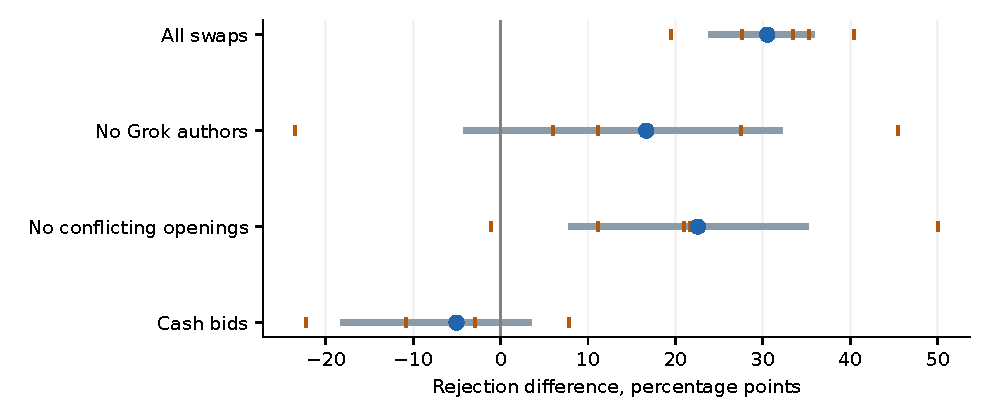
\includegraphics[width=.87\textwidth]{bargaining_stability.pdf}
\caption{Opening rejection differences between proposer-only and neither completion. Blue circles show pooled differences; orange ticks show the five seed-block differences; gray segments show the central 95\% of all 3,125 whole-block resamples. Different rows use different populations. The segments describe empirical reweighting stability, not a causal effect or independent confirmation.}\label{fig:stability}
\end{figure*}

These comparisons leave the mechanism open. Cash and property compensation, the proposer's identity and the recipient's portfolio differ across offers. Board list prices cannot resolve that problem because they omit complementarity and blocking value. We therefore use the record to establish the pattern of responses and examine strategic considerations directly in their own populations.

\subsection{Explicit consideration of rival development}
The separate semantic sample consists of seventy-four rejections of offers completing the recipient's group. Two LLM-assisted readings agree that 61 name a trade-linked consequence for the rival: 27/38 recipient-only and 34/36 both-completing offers. These populations are disjoint from the proposer-only/neither comparison above. They document expressed consideration of the rival, not an explanation for the swap/cash difference. Gemini and Grok contribute 56 of the agreed cases; G1 and G15 contribute 31. The concentration and reader identities matter when interpreting how representative those statements are.

\TranscriptTitle{g15}{Rejecting one's own completion because of the rival's}
At G15 turn 63, Sol offers two greens for Ventnor and \$100, completing both groups. Grok has \$333 and Sol \$730. Grok states:
\TranscriptQuote{fx-g15-refusal-note}
Sol subsequently offers the greens, Kentucky and \$250. Grok still refuses:
\TranscriptQuote{fx-g15-final-refusal}
The first offer leaves the stated \$830 and \$233. A full first layer on green costs \$600, although one legal house costs \$200. The objection concerns the rival's development, even when Grok would receive its own monopoly. All three offers fail. Eighteen turns later Grok's blockers pass to Gemini through bankruptcy; Sol never completes either group. This continuation reveals the stakes of withholding without identifying whether refusal improved Grok's chances.
\TranscriptSource{G15 d168--175, standard responses. The quoted public message occurs in the next counterparty request.}

\subsection{Prices and counteroffers express different choices}
Countering often retains the disputed exchange. In 111 counters to proposer-only completion offers, 79 preserve the entire noncash exchange while improving the counterer's cash. The corresponding figure for non-completing deed requests is 81/110. Repricing is common in both populations. Among unchanged-bundle concessions improving the recipient's cash, 9/58 proposer-only completion offers and 17/56 neither-completing deed requests are accepted. More money often leaves disagreement unresolved; these selected sequences do not identify a price response.

Single-deed asking prices are generally higher for completing buyers within seller and mortgage-status cells. More closely overlapping histories are mixed. Six same-game, same-seller, same-deed comparisons retain mortgage status: completing-buyer asks are higher in four, lower in one and equal in one. The seventh changes mortgage status and its ordering depends on the summary used. Time, buyer and negotiation history still differ. Appendix~\ref{app:comparisons} gives every pair rather than interpreting asking-price medians as an identified completion premium.

\TranscriptTitle{g2}{Pricing the buyer's development}
Opus holds two yellows and bids \$325 for Sol's Marvin Gardens. Sol responds:
\TranscriptQuote{g2-d124-price}
One turn earlier Sol asked Grok, which owned no yellow, for \$450 for that deed. Sol's note discusses Opus's remaining \$520 after the lower bid, but incorrectly calls it enough for nine yellow houses; it buys three. Opus calls \$450 final while privately retaining a \$475 ceiling. Sol refuses:
\TranscriptQuote{g2-d128-keep}
At turn 69 the exchange reverses direction. Opus has \$17 and sells its two yellows to Sol for two railroads and \$100. Sol builds, later liquidates those buildings, collects \$44 undeveloped rent and no developed yellow rent, then loses the group to Gemini through bankruptcy. The sequence shows explicit assessment of a competitor's future actions, a mistaken quantitative component and a later change in who can finance the group.
\TranscriptSource{G2 d119--128 and d197--198. Opus's first exchange uses standard responses; its later sale uses recovery.}

\TranscriptTitle{g19}{Accepting terms while correcting their justification}
Grok proposes Virginia and \$150 for States:
\TranscriptQuote{g19_d135_false_public}
Both deeds are pink. The same response's note says to abort and its assistant content names an end action, but the received proposal reaches Sol:
\TranscriptQuote{g19_d136_correction_accept}
The exchange executes and completes no group. Sol explicitly separates the false premise from acceptable terms. Grok's conflicting channels make the case unsuitable as evidence of one coherent deceptive plan, but the recipient's correction and acceptance are directly observed.
\TranscriptSource{G19 d135--136, standard responses. Sol's stored prompt contains the quoted false message.}
